% This question should answer the question: How did others try to solve the problem, and what did they miss?
% So, why is the problem not yet solved? In short, this should define the research gap of your work.
% For this, state-of-the-Art approaches should be described.
\chapter{Related Work}
\label{chap:related_work}

\begin{comment}
"Real-Time Performance and Response Latency Measurements of Linux Kernels on Single-Board Computers"
- das Paper vergleicht kontext switch latenzen zwischen linux und preempt-rt im speziellen auf einem Rpi3
- wurde jedoch vor 6.1 gemessen

Ich sollte mir noch eine Closed-Loop-Control implementierung anschauen, idealerweise in C oder auf einem FPGA
\end{comment}

The idea of using SBCs for embedded systems tasks is not something new.
The advantages of short test cycles, flexible implementations and a for the programmers familiar environment make general purpose processors seem very enticing for embedded systems.
This in combination with the spread of Raspberry Pis has led to similar research to our paper.

\section{Rasbperry Pi Research}

In \textit{Raspberry Pi performance analysis in real-time applications with the RT-Preempt patch} \cite{Rasp3}
the timing behavior of a Raspberry Pi 3 with the PREEMP-RT patch is investigated.
This includes a test polling a GPIO input,
a test for reaction times to hard- and software interrupts,
and a test running a ping-pong loop between two Rasbperry Pis with a one millisecond delay.

While these test are not directly comparable to our tests, as we mainly output things, while they tested input latencies, there is still very valuable information for us in this paper.
When we look at the test results from the timed loop test in Figure \ref{fig:rasp3}, we can see that they observed maximum latencies of three to eight times the minimum latencies.
If this translates into the worst-case latencies for our testing later it would render the Linux version unsuitable for our goal.

\begin{figure}
  \begin{center}
    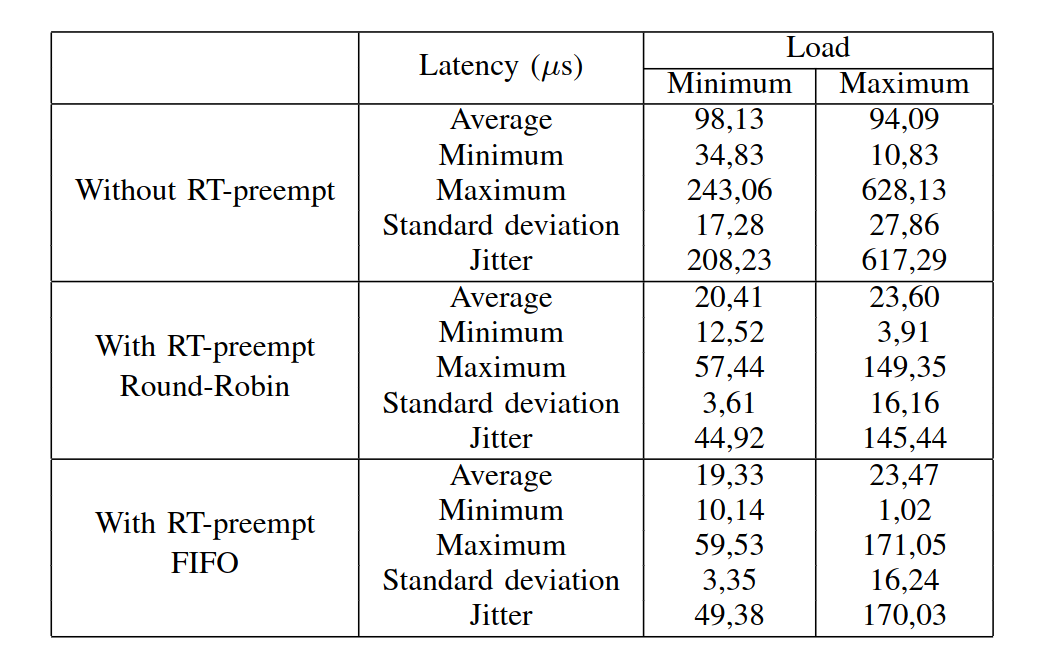
\includegraphics[width=.8\textwidth]{assets/Rasp3.png}
    \caption{Timed loop test results from \cite{Rasp3}}
    \label{fig:rasp3}
  \end{center}
\end{figure}

Almost identical research on the Raspberry Pi 3 has been done in \textit{Real-Time Performance and Response Latency Measurements of Linux Kernels on Single-Board Computers} \cite{computers10050064}.
This paper also used the ping-pong loop between two Raspberry Pis for the reaction time measurement.
There are some small differences to the former paper:
\begin{enumerate}
  \item For comparison the paper includes the Beagle Bone Black SBC
  \item The kernels tested are the far older 4.14 and 4.19 kernels
  \item The paper also considers multiple Linux distributions (Ubuntu, Arch Linux, and Debian), which can affects the tools and flags to compile the kernel.
\end{enumerate}
Interesting here are the results in comparison with the former paper, for the Debian version, which had the newest kernel, the minimum response time was 40$\mu$s and the maximum 90 $\mu$s.
One possible explanation for the far higher latencies than in the former paper could be the comparatively old kernel version.

Similarly, \textit{A Performance Evaluation of Embedded Multi-core Mixed-criticality System Based on PREEMPT RT Linux} \cite{Rasp4},
tests latency and throughput characteristics with PREEMPT-RT on the Raspberry Pi 4.
Although this is the same hardware as we use, there are some important differences:\\
They propose a approach splitting real-time and best-effort tasks by running the best-effort tasks on a virtualized unmodified Linux kernel.\\
They measure task wake-up times using cyclitest, a tool developed together with PREEMPT-RT, while we test for our specific use case and compare to a bare-metal version.\\

During the writing of this thesis the new Raspberry Pi 5 got released, with a faster processor and more IO capabilities.
Does this mean that our research is already outdated?\\
Not necessarily, similar to the Raspberry Pi 4, the Raspberry Pi 5 suffers from supply bottlenecks,
as demand outpaces the production capacity of the Raspberry Pi foundation, making Raspberry Pi 4s cheaper and more readily available.
Additionally many improvements of the Raspberry Pi 5 are more benefitial for server style tasks as opposed to embedded systems:
\begin{itemize}
  \item the additional IO capabilities of the Pi 5 are just more and faster PCIe lanes, which has very little relevance for embedded systems and especially our use case.
  \item the addition of a real-time clock to have persistent time across reboots is of little importance for our use case.
  \item the faster processor may only benefit our system marginally, as the IO times on the Pi 4 are already significantly slower than the computations.
\end{itemize}

Still, there will be some benefits to the Pi 5 and there is already some preliminary research on its real-time capabilities.
\textit{A Preliminary Assessment of the real-time capabilities of Real-Time Linux on Raspberry Pi 5} \cite{Rasp5} examines the Raspberry Pi 5's real-time capabilities using cyclitest,
similar to \textit{A Performance Evaluation of Embedded Multi-core Mixed-criticality System Based on PREEMPT RT Linux} \cite{Rasp4}.
In Figure \ref{fig:rasp4} and \ref{fig:rasp5}, we compare the results of the two papers.
This comparison is interesting because according to these results, the Pi 4 is better at real-time operations at the moment.
This may be because Linux is not yet fully optimized for the architecture of the new bcm2712 processor.

\begin{figure}
  \begin{center}
    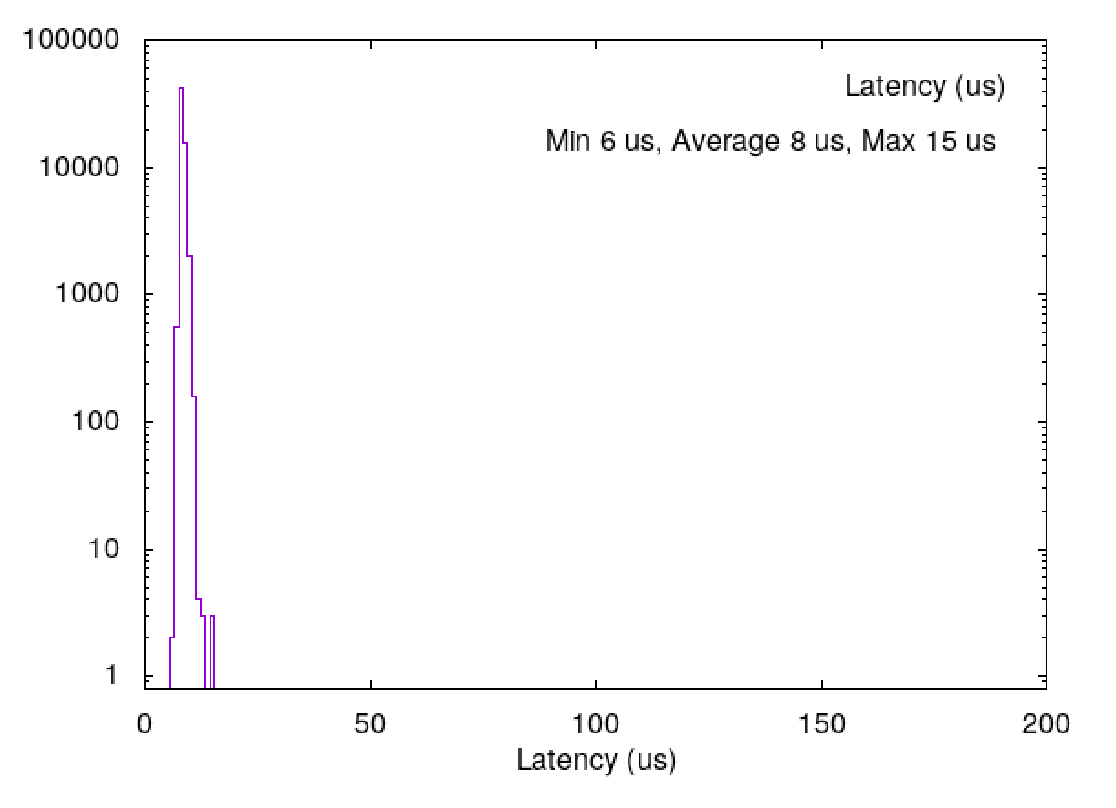
\includegraphics[width=.8\textwidth]{assets/Rasp4.png}
    \caption{Kernel scheduling latency on the Raspberry Pi 4 measured with cyclitest \cite{Rasp4}}
    \label{fig:rasp4}
  \end{center}
\end{figure}

\begin{figure}
  \begin{center}
    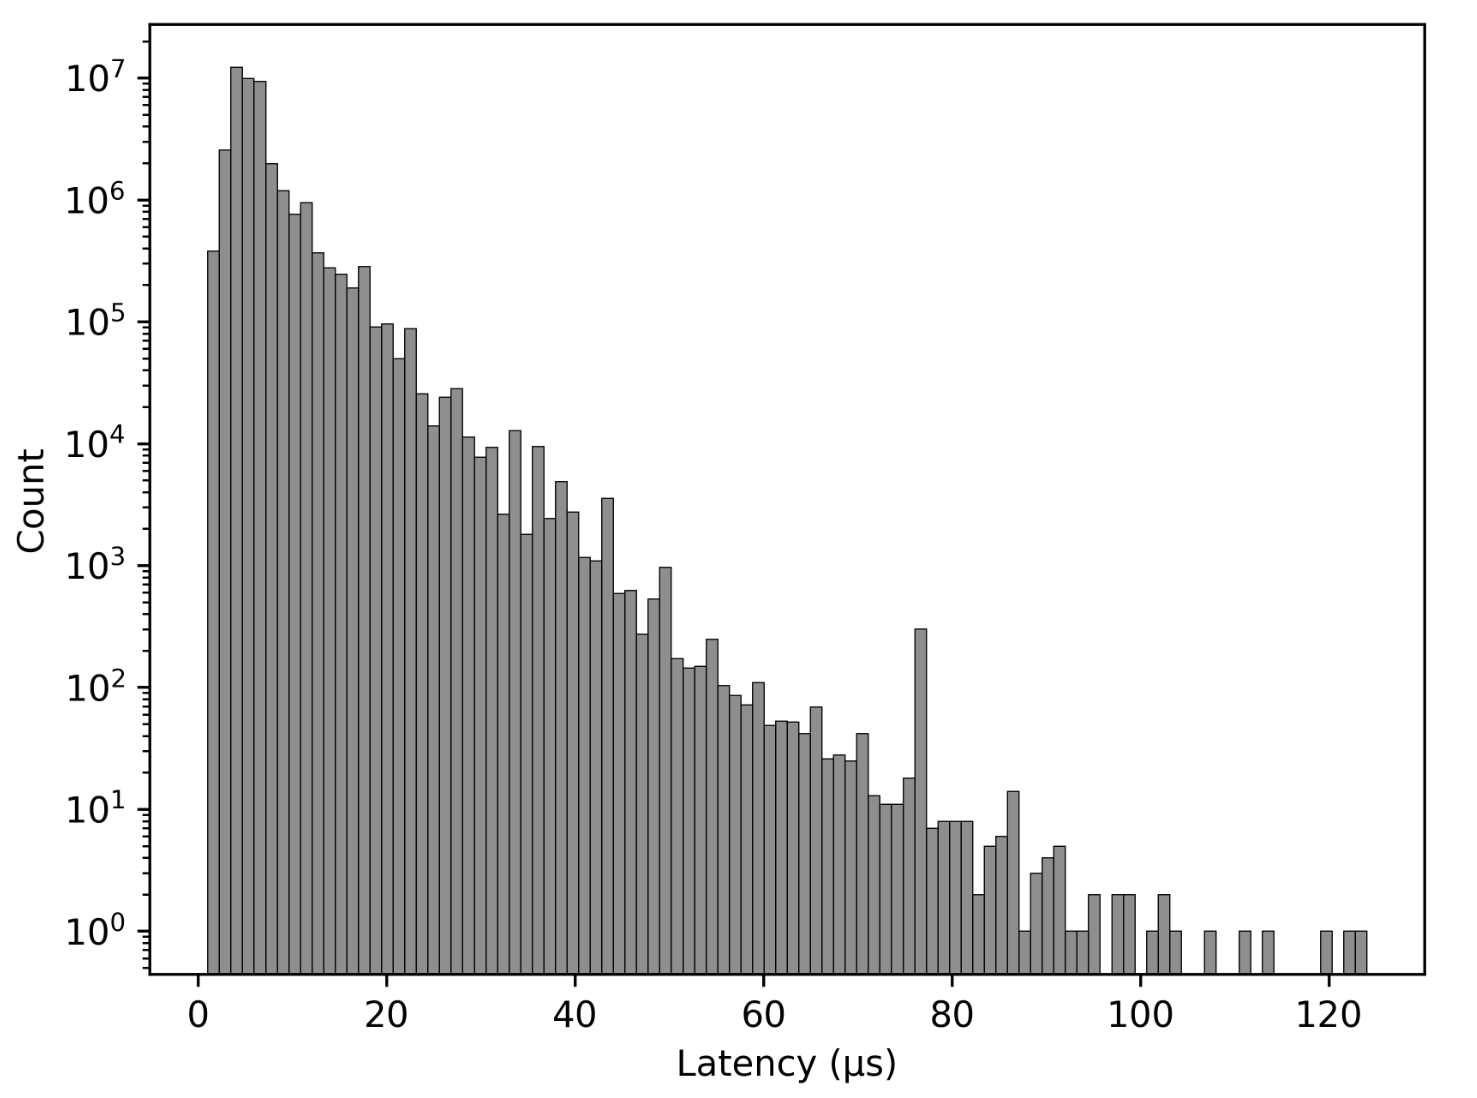
\includegraphics[width=.8\textwidth]{assets/Rasp5.png}
    \caption{Kernel scheduling latency on the Raspberry Pi 5 measured with cyclitest \cite{Rasp5}}
    \label{fig:rasp5}
  \end{center}
\end{figure}

\section{Rust for embedded systems}

Rust's usage for embedded systems is very active research area.
The research can be roughly split into two categories:
\begin{enumerate}
  \item Evaluating new approaches that are made possible by Rust's modern features, like the borrow checker and zero sized types.
  \item Evaluating how Rust solves old problems with already known solutions.
\end{enumerate}

In the first category, research into embedded operating systems is a very common target.
A very prominent example of this is the Tock RTOS \cite{tock}, a Rust written OS kernel with a strong focus on security.
For this RTOS alone, there are already papers investigating the general architecture \cite{tock2}, the limitations \cite{theft}, possible solutions \cite{tock3}, and the security model \cite{tock4}.

But, since our research clearly falls into the second category, we will focus on that.
For an up to date overview of the general state of Rust, \textit{Rust for Embedded Systems: Current State, Challenges and Open Problems} \cite{sharma2023rustembeddedsystemscurrent} is a recent paper that focusses on a general overview.
The important part for us here is their second research question:\\
Interoperability of RUST. How well can RUST interoperate with existing C codebases, and what are its challenges?

Because this is closely related to our own Rust research this opens up a few questions.
How did they investigate the question, What did they find, and how does it relate to our research?

For this research they developed a simple Rust application on top of FreeRTOS,
a common RTOS written in C, and the same application in C built on top of a Rust port of FreeRTOS.
We will later only look at the direction Rust on top of C.
The results of their research are two findings:
\begin{quotation}
  Significant development effort is required to engineer a C embedded application on top of RUST RTOSes.
\end{quotation}
\begin{quotation}
  It is easy to convert a self-contained, embedded system component of C RTOS into RUST.
\end{quotation}

There is one big difference in our research however, that could lead to a different conclusion than they have;
Our project will be built upon the Circle library, which is a C++ library, that provides a mostly C-style API,
but has some functions that make use of inheritance.